\section{Cascade Inverse Kinematics}
\label{appendix:CIK}

The Cascade Inverse Kinematics (CIK) algorithm maps a deformed canonical sphere to embodiment-specific joint configurations $\mathbf{q}$ for arbitrary robotic hands. Its objective is to position the hand surface points as close as possible to their corresponding locations on the input deformed sphere while respecting kinematic constraints. These correspondences are established during automatic sphere creation and surface projection (Section \ref{sec:surface_correspondence} and Fig. \ref{fig:surface_correspondence}).

Traditional numerical inverse kinematics solvers are computationally expensive and unsuitable for real-time dexterous control. In contrast, CIK exploits the geometric structure of the Unified Hand Action Space together with a cascaded decomposition of joint responsibilities. In our real-world setup, the complete CIK pipeline runs at approximately \textbf{150 Hz}. In practice, CIK was never the runtime bottleneck. The dominant sources of latency were serial communication with the LEAP hand and AprilTag-based object pose estimation. We provide more details of the CIK algorithm below.

\paragraph{Joint Classification.}
We classify every joint of a robotic hand into one of two categories according to its dominant geometric effect on the fingertip position in the sphere coordinate frame. Classification is performed once per hand from its URDF in a base open-hand configuration. For each joint, we sweep it across its full range of motion while keeping all other joints fixed, and we record the resulting changes in the fingertip's spherical coordinates $(\theta, \phi, r)$ via forward kinematics. In cases where a joint's rotation axis points toward the fingertip, we partially flex the remaining joints of the finger and repeat the sweep to determine its dominant effect. Joints are then categorized as follows:

\begin{itemize}
    \item \textbf{Lateral joints} are those that predominantly affect the azimuthal angle $\theta$ of the fingertip, producing side-to-side finger motion.
    \item \textbf{Encompassing joints} are those that most strongly influence the radial distance $r$ and polar angle $\phi$ of the fingertip, allowing the finger to conform to the sphere surface.
\end{itemize}

This joint classification procedure is illustrated in Fig.~\ref{fig:joint_class}, where a joint is automatically classified according to the effect of the joint change on the position of the fingertip. Because the fingers are kinematically independent in the UHAS formulation, lateral and encompassing joints are solved sequentially but \emph{independently for each finger}.

\begin{figure}[h]
\centering
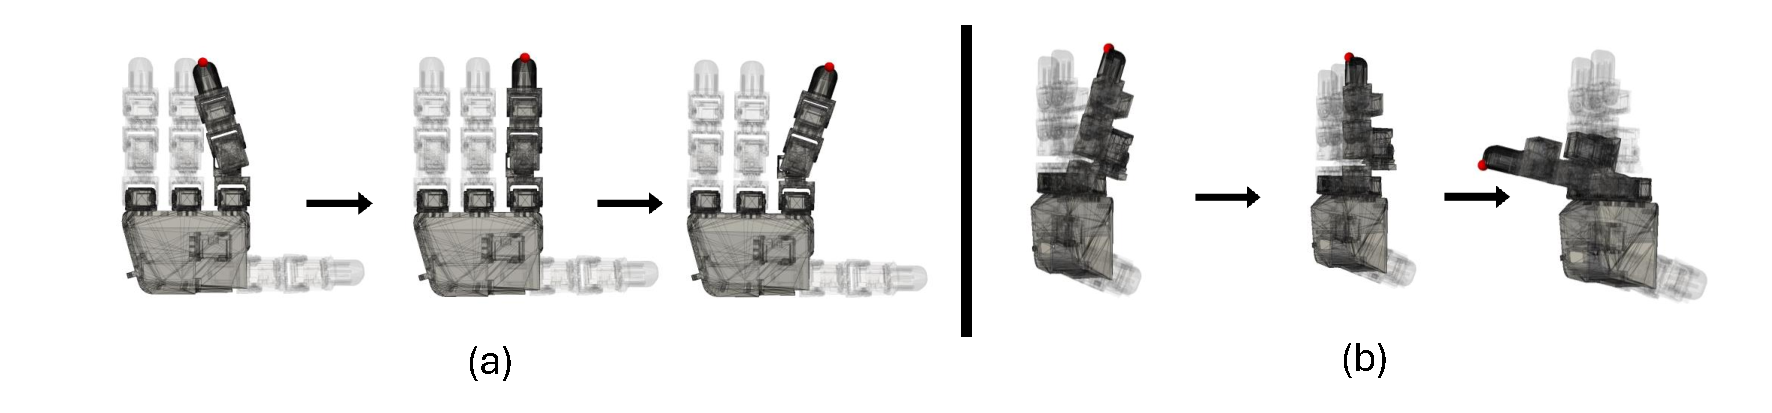
\includegraphics[width=\linewidth]{figures/joint_class.pdf}
\vspace{-2mm}
\caption{Illustration of the joint classification procedure in the Cascade Inverse Kinematics (CIK) algorithm. (a) Classification of lateral joint based on their effect on the fingertip azimuthal angle $\theta$. (b) Classification of encompassing joints based on their effect on the fingertip radial distance $r$ and polar angle $\phi$.}
\label{fig:joint_class}
\vspace{-2mm}
\end{figure}

\paragraph{Lateral Joint Mapping via Lookup Table.}
To enable fast lateral finger control, we precompute a lookup table for every lateral joint with the following steps:
\begin{enumerate}
    \item Sweep the lateral joint across its full range of motion in uniform steps.
    \item For each sampled value, fix the lateral joint and solve the encompassing joints on the \emph{undeformed} reference sphere.
    \item Record the resulting azimuthal angle $\theta_{\text{fingertip}}$ of the corresponding fingertip (surface point) on the canonical sphere frame.
    \item Store the mapping: lateral joint value $q_{\text{lateral}} \mapsto \theta_{\text{fingertip}}$.
\end{enumerate}

During inference, the policy outputs a lateral deformation $\Delta\theta$ for the driving plane aligned with the finger. We compute the fingertip target angle
\[
\theta_{\text{fingertip}} = \theta_{\text{initial}} + \Delta\theta,
\]
where $\theta_{\text{initial}}$ corresponds to the neutral (middle-of-range) pose of the finger. The precomputed lookup table directly yields the target lateral joint value $q_{\text{lateral}}$. The table is built offline once per hand and provides constant-time lateral solving at runtime.

\paragraph{Encompassing Joint Cascade.}
After the lateral joints have been set, we solve the encompassing joints sequentially in proximal-to-distal order along each finger’s kinematic chain. For each encompassing joint $i$, we first use forward kinematics with the already computed parent joint values to transform the target sphere surface points associated with joint $i$ and all its descendant links into the local coordinate frame of joint $i$. We then directly compute the joint angle that places both the current joint’s surface correspondences and those of its children onto the deformed sphere surface, as illustrated in Fig.~\ref{fig:CIK}. Because each joint is solved exactly once in a single forward pass with no iterative numerical optimization, the cascade remains extremely lightweight. This cascaded procedure progressively conforms the finger geometry to the target sphere deformation while preserving kinematic feasibility. The final joint configuration $\mathbf{q}$ is the output of the complete CIK algorithm.

\paragraph{Sphere Controller.}
By combining the compact sphere-deformation action space with CIK we obtain the complete \emph{Sphere Controller}. At every policy timestep the actor predicts driving-plane rotations ($\Delta\theta$) and driving-vector displacements ($\Delta r$). These parameters define a deformed sphere that is passed to CIK, which returns embodiment-specific joint positions $\mathbf{q}$ for the low-level controller. The lightweight sequential structure of CIK enables real-time execution across diverse robotic hands while remaining fully decoupled from any particular morphology. This design is central to the strong zero-shot transfer and rapid finetuning performance reported in Section~\ref{sec:exp}.


\section{Policy Details}
\label{appendix:training}
We provide implementation details of the reinforcement learning policies trained using the Unified Hand Action Space (UHAS). We describe the homogeneous observation space and the sphere-based action parameterization that enable effective cross-embodiment learning as well as training hyperparameters, domain randomization, and reward details in Appendix~\ref{appendix:training_rl}. 

A key requirement for training a single policy across robotic hands with different kinematic structures is the normalization of both \emph{observation and action spaces}. Standard observation formulations for in-hand manipulation include goal rotation, object pose, object linear and angular velocities, the quaternion difference to the target orientation, joint positions and velocities, and previous actions. However, raw joint values cannot be used directly because their semantic meaning and numerical ranges vary significantly across embodiments, hindering cross-embodiment transfer. We therefore represent hand configuration through points defined via surface correspondences on the finger chains (Section~\ref{sec:surface_correspondence}).

\paragraph{Sphere Observation Space.}
We construct homogeneous observations from points sampled along each finger rather than from raw joint values. For every finger, we first discretize the kinematic chain into 7 equally spaced points from root to fingertip. The parent joint of each sampled point is determined by its closest surface correspondence on the canonical sphere (Section~\ref{sec:surface_correspondence}). Positions of these points under the current joint configuration are obtained via forward kinematics. Linear and angular velocities of the points are computed using the corresponding Jacobians evaluated at the current joint configuration and joint velocities.

For all policies presented in the main paper we retain only two points per finger: the middle point and the fingertip. This choice provides a compact yet informative representation of finger configuration while remaining consistent across hands with different numbers of fingers. For 4-finger hands we duplicate the ring-finger observations to preserve dimensional consistency with 5-finger embodiments. All point positions and velocities are expressed in the canonical sphere coordinate frame (Fig.~\ref{fig:sphere_construction}) and normalized by the hand-specific sphere radius $r$. An illustration of the homogeneous observation points across different hands is shown in Fig.~\ref{fig:Homogeneous observations}. A detailed ablation on the number of observation points is provided in Appendix~\ref{appendix:ablations}.

\begin{figure}[h]
\centering
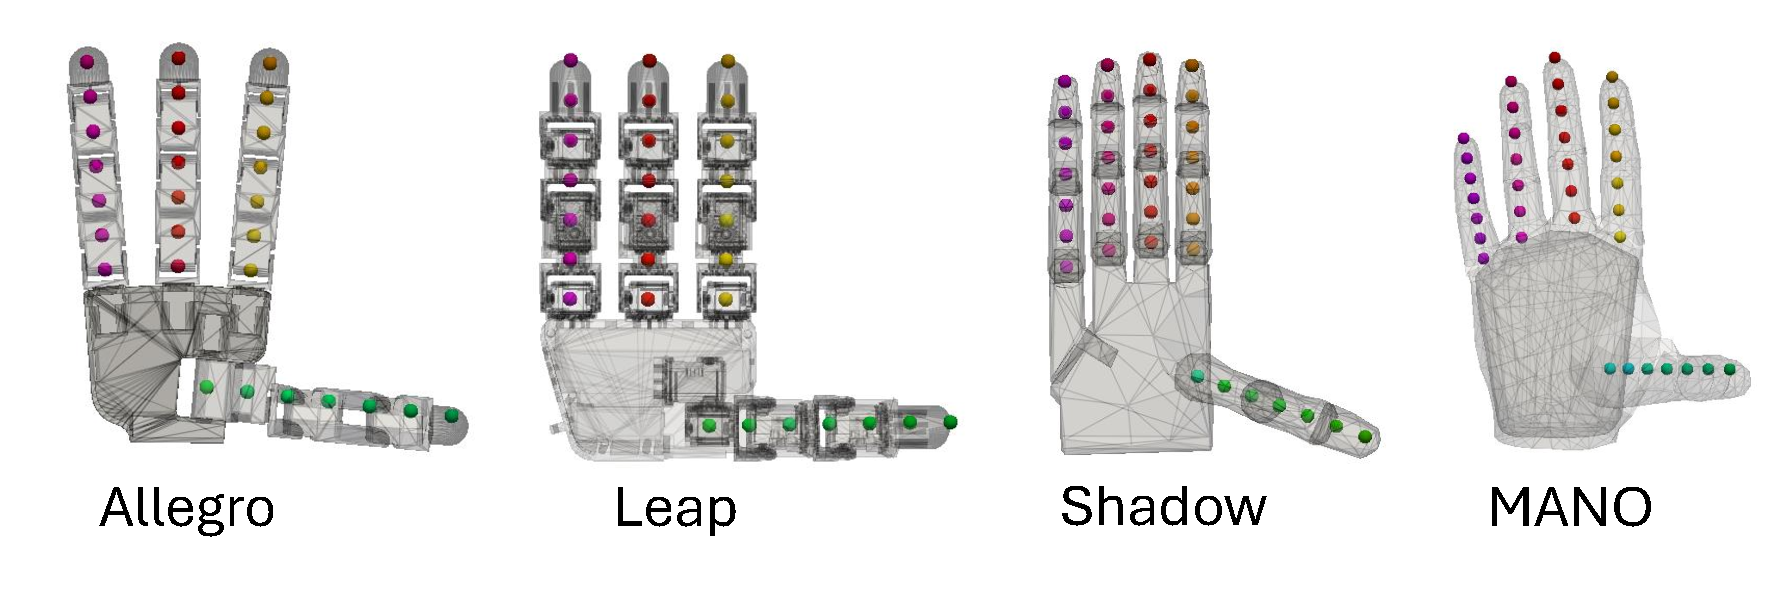
\includegraphics[width=\linewidth]{figures/homogeneous_obs.pdf}
\vspace{-2mm}
\caption{Homogeneous observations across different robotic hands.}
\label{fig:Homogeneous observations}
\vspace{-2mm}
\end{figure}

\paragraph{Sphere Action Space.}
Actions are defined in the sphere deformation space introduced in Section 3.3. Each action consists of lateral deformations $\Delta\theta$ applied to a set of driving planes and radial deformations $\Delta r$ applied to driving vectors within those planes. We attach one driving plane per fingertip and align its initial azimuthal angle with the corresponding fingertip $\theta$ on the canonical sphere. To enable a unified policy across both 4-finger and 5-finger hands while preserving independent actuation of the fifth finger, we introduce an additional driving plane at the ring-finger azimuthal position for all 4-finger embodiments. When computing deformations in the ring finger, the $\Delta\theta$ and $\Delta r$ actions of the duplicated plane are averaged before interpolation.

Lateral actions are bounded to the extremal values stored in the precomputed lookup tables of each hand. We employ two driving vectors per plane, positioned at equally spaced polar angles $\phi = 60^\circ$ and $\phi = 120^\circ$, with radial displacements defined over the interval $[-2, 2]$. Prior to invoking the Cascade Inverse Kinematics (CIK) algorithm, we discard all sphere points whose radial coordinate $r$ is negative. If an encompassing joint has no reachable points remaining after this filtering step, the joint is commanded to its fully closed configuration. This design choice was made after observing that permitting negative radial deformations substantially improves performance on the highly dynamic cube reorientation task, as it allows the policy to close fingers rapidly during aggressive reposing maneuvers. An ablation study on the number of driving vectors per plane is provided in Appendix~\ref{appendix:ablations}.

\subsection{Training}
\label{appendix:training_rl}

\paragraph{Hyperparameters.}
All models were trained on a single NVIDIA A5000 GPU using the RSL-RL implementation of Proximal Policy Optimization (PPO) \cite{schwarke2025rslrl}. Training is performed in the custom NVIDIA Isaac Lab Cube Reposing environment \cite{mittal2025isaaclab} running on Isaac Sim 4.5.0 with the PhysX physics simulator. The complete set of PPO training hyperparameters is summarized in Table~\ref{tab:ppo_hyperparameters}.

\begin{table}[h]
\centering
\caption{PPO training hyperparameters.}
\label{tab:ppo_hyperparameters}
\vspace{-2mm}
\begin{tabular}{ll}
\toprule
\textbf{Hyperparameter}              & \textbf{Value}                  \\
\midrule
\multicolumn{2}{l}{\textit{Runner Configuration}} \\
\midrule
Num. steps per environment           & 16                              \\
Empirical normalization              & True                            \\
\midrule
\multicolumn{2}{l}{\textit{Policy Network (Actor \& Critic)}} \\
\midrule
Hidden layer dimensions              & $[512, 512, 256, 128]$          \\
Activation function                  & ELU                             \\
Initial action noise std.            & $1.0$                           \\
\midrule
\multicolumn{2}{l}{\textit{PPO Algorithm}} \\
\midrule
Learning rate                        & $5.0 \times 10^{-4}$            \\
Learning rate schedule               & adaptive                        \\
Clip parameter                       & $0.2$                           \\
Entropy coefficient                  & $0.005$                         \\
Num. learning epochs                 & $5$                             \\
Num. mini-batches                    & $4$                             \\
Value loss coefficient               & $1.0$                           \\
Use clipped value loss               & True                            \\
Discount factor ($\gamma$)           & $0.99$                          \\
GAE parameter ($\lambda$)            & $0.95$                          \\
Desired KL divergence                & $0.016$                         \\
Max. gradient norm                   & $1.0$                           \\
\bottomrule
\end{tabular}
\vspace{-2mm}
\end{table}

\paragraph{Reward Function.}
We adopt the reward formulation from the original NVIDIA Isaac Lab Reposing Cube environment. To discourage embodiment-specific exploitation—such as policies that rely predominantly on lateral joint motion while underutilizing encompassing joints—we augment the original reward with two additional regularization terms. These terms penalize deviations of the lateral and encompassing joint positions from a reference joint configuration. Let $d$ denote the object-to-goal distance and $r_{\text{rot}}$ the orientation alignment reward. Let $p_{\text{lat}}$ and $p_{\text{rad}}$ denote the lateral and encompassing joint position penalties, respectively. The scalar reward at each timestep is then computed as
\begin{equation}
    r = w_d \, d + w_r \, r_{\text{rot}} + w_{\text{lat}} \, p_{\text{lat}} + w_{\text{rad}} \, p_{\text{rad}} + b_{\text{success}} + p_{\text{fall}},
\end{equation}
where $b_{\text{success}}$ is a large positive bonus awarded upon reaching the goal within tolerance of 0.1 radians, and $p_{\text{fall}}$ is a negative penalty applied when the object falls. The reward scales used during training are reported in Table~\ref{tab:reward_scales}.

\begin{table}[h]
\centering
\caption{Reward scales used during training.}
\label{tab:reward_scales}
\vspace{-2mm}
\begin{tabular}{ll}
\toprule
\textbf{Reward Term}                              & \textbf{Scale}          \\
\midrule
Object-to-goal distance ($w_d$)                   & $-10.0$                 \\
Orientation alignment ($w_r$)                     & $1.0$                   \\
Reach goal bonus ($b_{\text{success}}$)           & $250$                   \\
Fall penalty ($p_{\text{fall}}$)                  & $-100$                  \\
Lateral joint position penalty ($w_{\text{lat}}$) & $-0.016$                \\
Encompassing joint position penalty ($w_{\text{rad}}$) & $-0.004$           \\
\bottomrule
\end{tabular}
\vspace{-2mm}
\end{table}
\paragraph{Domain Randomization.}

\begin{table}[h]
\centering
\caption{Domain randomization ranges applied during training.}
\label{tab:domain_randomization}
\vspace{-2mm}
\small
\begin{tabular}{ll}
\toprule
\textbf{Parameter}                              & \textbf{Randomization Range}          \\
\midrule
\multicolumn{2}{l}{\textit{Object Properties}} \\
\midrule
Object scale                                    & $[0.9, 1.1] \times$ nominal         \\
Object mass                                     & $[0.8, 1.2] \times$ nominal         \\
Object static friction                          & $[0.2, 0.3]$                        \\
Object dynamic friction                         & $[0.15, 0.25]$                      \\
\midrule
\multicolumn{2}{l}{\textit{Robot Properties}} \\
\midrule
Robot mass                                      & $[0.9, 1.1] \times$ nominal         \\
Robot static / dynamic friction                 & $[0.75, 1.0]$                       \\
Joint friction                                  & $[0.9, 1.1] \times$ nominal         \\
Joint armature                                  & $[1.00, 1.05] \times$ nominal       \\
Joint effort limits                             & $[0.9, 1.1] \times$ nominal         \\
Joint stiffness                                 & $[0.75, 1.25] \times$ nominal       \\
Joint damping                                   & $[0.75, 1.25] \times$ nominal       \\
\midrule
\multicolumn{2}{l}{\textit{Hand Pose \& Action Space}} \\
\midrule
Hand base inclination                           & $15^\circ \pm 5^\circ$              \\
Driving vector azimuthal angle ($\phi$)         & $\pm 15^\circ$                      \\
\bottomrule
\end{tabular}
\vspace{-2mm}
\end{table}

We utilize domain randomization during policy training. These randomization strategies proved beneficial for improving cross-embodiment generalization. Randomizing the hand base inclination discouraged policies from relying on specific cube-palm interaction dynamics, such as assuming the cube would slide or settle into particular regions of the palm. Object scale randomization helped mitigate finger entrapment issues arising from differences in finger geometry across embodiments. Additionally, randomizing the driving vector azimuthal angle $\theta$, joint effort limits, and PD gains altered the in-distribution dynamics of each hand which improved generalization, particularly across certain hands. An ablation study examining the contribution of these randomization components is provided in Appendix~\ref{appendix:ablations}. Table~\ref{tab:domain_randomization} shows the details of the domain randomization used for training. Note that the domain randomization strategy used for real-world deployment differed from the one described in this section. Details of real-world deployment are provided in Appendix~\ref{appendix:sys_ID}.




\section{Cube Pose Estimation}
\label{appendix:cube_pose}

We track a 3D-printed cube based on an open source design~\cite{park2026aprilcube}. Each of its six faces carries four distinct \texttt{tag36h11} AprilTags~\cite{apriltag} (24 tags total). One or two Intel RealSense cameras each stream a rectified infrared image at $848\times480$ pixels and 60 Hz. A second camera viewpoint increases the number of visible tags on the cube that are not occluded by the hand. We also placed the hand in a well-lit location allowing for shorter exposure time to reduce motion blur during fast reorientation movements.

Each visible tag is localized independently via perspective-n-point pose estimation using its four corners and the camera intrinsics. Detected tags are only published if the Hamming decoded value is zero and the decision margin is at least 50. A separate standalone tag is placed at a known location on the base mount and serves as a common reference frame.

In the dual-camera configuration, messages timestamped within 100 ms of each other are paired. The transformation from the secondary to the primary camera frame is estimated from tags visible in both camera views. In the case of duplicate tags which both cameras see, the tag with the higher detection margin will be kept. Given the final set of visible tags, the cube pose is calculated by chaining the camera-to-tag pose with the calibrated cube-to-tag transform. Estimates whose translation deviates by more than 10 mm from the median or whose orientation deviates by more than 0.075 rad from a consensus quaternion are dropped. The remaining estimates are fused by their mean position and hemisphere-aligned quaternion averaging. The cube pose is published only when at least three separate tags are visible.

\section{System Identification}
\label{appendix:sys_ID}

To enable reliable sim-to-real transfer, we performed system identification on the complete real-world hardware setup, including the LEAP Hand, its actuators, and the communication interface. Due to the limited serial communication bandwidth of the LEAP Hand, we operate the policy at a control frequency of 20 Hz during training and real-world deployment.

% We model the servo control law as current $I(t) = K_p \Delta\theta(t) - K_d \Delta\dot{\theta}(t)$, where $\Delta\theta(t)$ is the joint error, and $K_p$ and $K_d$ are the PD control gains. However, directly mapping this formulation to the implicit PD torque actuators in simulation did not produce motion profiles consistent with real-world behavior. To address this discrepancy, we identified the effective proportional and derivative gains $K_p$ and $K_d$ directly from the physical LEAP Hand. We collected data by commanding random target positions under varying gain settings and solved for the gains that best reproduced the observed joint position, velocity and current readings. The identified values differed substantially from the manufacturer specifications, particularly in the damping term. We attribute this difference to the current-based position control mode used by the motors. \yu{Do you use these identified values in simulation training? We need to write about what the result of the system identification.}

We model the servo control law of the LEAP Hand as $\text{current}(t) = K_p \Delta\theta(t) - K_d \Delta\dot{\theta}(t)$, where $\Delta\theta(t)$ denotes the joint position error. Directly mapping this current-based formulation to the implicit PD torque actuators available in simulation did not reproduce the motion observed on the physical robot. To resolve this mismatch, we performed system identification on the LEAP Hand by commanding random target positions while varying the commanded $K_p$ and $K_d$ gains. From the recorded joint position, velocity, and current trajectories, we solved for the effective gains that best matched the recorded data. The identified values were subsequently used when training policies intended for real-world deployment.

The system identification revealed that the LEAP Hand motors behave as a nearly undamped system, with damping having a negligible effect on the observed dynamics. Furthermore, the effective proportional gain $K_p$ differed from the manufacturer specifications: approximately $0.0786~\text{Nm/rad}$ per 100 motor units. The effective derivative gain $K_d$ was found to be approximately $0.0014~\text{Nm/(rad/s)}$ per 100 motor units. We attribute these discrepancies primarily to the current-based position control mode employed by the motors.

By monitoring the motor state during operation, we observed that the LEAP Hand reliably enforces its internal velocity limits. Accordingly, we introduced velocity limits in simulation when training models intended for real-world deployment. These limits were themselves randomized during training to improve robustness.

\subsection{Training for Real-World Deployment}

For models deployed on the physical robot, we increased the range of domain randomization compared to simulation-only training. In addition to the randomization parameters described in Table~\ref{tab:domain_randomization}, we randomized the velocity limits applied in simulation. We also adopted an asymmetric actor-critic architecture: the actor receives only positional information of the object and hand joints, while the critic has access to the full state, including linear and angular velocities of the object and hand. This design encourages the actor to learn policies that rely primarily on position feedback, which is more reliable under real-world sensing and communication noise.

\subsection{Deployment on the Physical LEAP Hand}

During real-world operation, we observed that serial communication with the LEAP Hand was unreliable, with frequent missed reads and writes. To mitigate this, we implemented additional software-level communication management to improve reliability. Despite these measures, certain motor state readings consistently failed through the manufacturer API.

We further limited the range of several joints on the physical hand. This was necessary because the joints exhibited overshoot and because the structural components of the LEAP Hand are relatively deformable under load. We also imposed a lower velocity limit than the hardware maximum to reduce overshooting observed during fast motions.

Finally, we observed that the fingers of the LEAP Hand gradually became loose after repeated use. To improve mechanical stability, we designed and 3D-printed a reinforced base that secures the root joints of the index, middle, and ring fingers using additional screws. We also observed significant deformation at the thumb root joint and therefore designed a custom attachment for it. Both the reinforced finger base and the thumb attachment will be released publicly alongside the paper.


\section{Additional Ablation Studies}
\label{appendix:ablations}

We present additional ablation studies on two key design choices in our method: the number of homogeneous observation points per finger and the number of driving planes in the Unified Hand Action Space. In addition, we present an ablation study on domain randomization.

\paragraph{Ablation on Observation Points.}
We ablate the number of homogeneous observation points per finger. Fig.~\ref{fig:Homogeneous observations} illustrates the full set of candidate points distributed along each finger. From these points, we select different subsets as observations: one point at the fingertip, two points consisting of the finger midpoint and fingertip, or three and four equally spaced points along the finger. All models were trained amd tested on the four hands using one NVIDIA A5000 GPU while keeping all other components fixed. As reported in Table~\ref{tab:observation_ablation}, increasing the number of observation points provides only marginal improvements in success rate and average consecutive reorientations. These gains become negligible when domain randomization is applied, while training time and inference cost increase. We therefore use two observation points per finger (midpoint and fingertip) in our final models, as this configuration achieves a favorable trade-off between performance and computational efficiency. Additional details regarding the construction of the homogeneous observations are provided in Appendix~\ref{appendix:training}.

\begin{table}[h]
\centering
\caption{Ablation on the number of homogeneous observation points per finger.}
\label{tab:observation_ablation}
\vspace{-2mm}
\setlength{\tabcolsep}{6pt}
\begin{tabular}{lcccc}
\toprule
\textbf{\# Observation Points} 
& \textbf{1} 
& \textbf{2} 
& \textbf{3} 
& \textbf{4} \\
\midrule
\textbf{Success Rate} 
& 98.8
& 98.7
& 99.0
& \textbf{99.1} \\

\textbf{\# Reorientations} 
& 9.3 $\pm$ 2.1
& 9.3 $\pm$ 2.0
& 9.4 $\pm$ 1.8 
& \textbf{9.5 $\pm$ 1.8} \\

\textbf{Training Time (h)} 
& 4.9
& \textbf{4.5}
& 4.8
& 4.7 \\
\bottomrule
\end{tabular}
\vspace{-2mm}
\end{table}
\paragraph{Ablation on Driving Planes.}
Additionally, we ablate the number of driving planes in the Unified Hand Action Space (UHAS). For the non-zero-shot models, we train and evaluate each hand using either the standard 5-plane UHAS or a 4-plane variant. The 4-plane version is constructed identically to our merging procedure for 4-finger hands: we compute the average deformation of the ring and pinky planes and then interpolate the canonical sphere points as usual. For the zero-shot models, we train on the other three hands and deploy using the 4-plane UHAS (again merging the ring and pinky planes). Consequently, the 4-plane zero-shot policies move the ring and pinky fingers in a coupled manner.

As shown in Table~\ref{tab:driving_planes_ablation}, using 4 or 5 driving planes yields very similar performance. Interestingly, the Shadow hand even achieves slightly better results with 4 planes than with 5. We attribute this to the fact that the pinky finger is rarely used to solve the cube reposing task; therefore, removing its dedicated driving plane has a negligible impact on task performance.

We attempted to train models using only 3 driving planes. However, these models were unable to reliably solve the reposing task, and training failed to converge to meaningful policies. This indicates that a minimum level of action-space expressiveness is required for stable learning on this task.

It is important to note that the small difference observed between 4 and 5 planes may be specific to this reposing task, the particular reward formulation and the reference cube position used. These factors had a significant influence on hand behavior during training. Therefore, the negligible impact of removing the fifth plane should not be assumed to hold for other manipulation tasks or reward designs.

\begin{table}[h]
\centering
\caption{Ablation on the number of driving planes.}
\label{tab:driving_planes_ablation}
\vspace{-2mm}
% \scriptsize
\setlength{\tabcolsep}{8pt}
\begin{tabular}{lcc}
\toprule
\textbf{\# Driving Planes} & \textbf{4} & \textbf{5} \\
\midrule
Shadow                  & \textbf{99.5 / 9.7 $\pm$ 1.5} & 99.3 / 9.6 $\pm$ 1.6 \\
Shadow (Zero-shot)      & \textbf{86.9 / 4.8 $\pm$ 3.8} & 85.7 / 4.4 $\pm$ 3.7 \\
MANO                    & 99.6 / 9.8 $\pm$ 1.3 & \textbf{99.8 / 9.9 $\pm$ 1.0} \\
MANO (Zero-shot)        & 98.0 / 8.7 $\pm$ 2.9 & \textbf{98.1 / 8.9 $\pm$ 2.6} \\
\bottomrule
\end{tabular}
\vspace{-2mm}
\end{table}

\paragraph{Ablation on Domain Randomization.}
We evaluate the impact of domain randomization on zero-shot cross-embodiment generalization. For each hand, we train models on the other three hands and evaluate zero-shot transfer performance. We compare models trained with and without randomization of PD gains, joint effort limits, object scale, and driving vector polar angle $\phi$. Table~\ref{tab:randomization_ablation} reports the results across all four hands. Randomization during training consistently improves zero-shot transfer, particularly for hands with larger morphological differences from the training set.

\begin{table}[h]
\centering
\caption{Zero-shot performance with and without domain randomization (PD gains, effort, object scale, and vector $\phi$). Results reported as Success Rate / Average Consecutive Reorientations $\pm$ std.}
\label{tab:randomization_ablation}
\vspace{-2mm}
% \scriptsize
\setlength{\tabcolsep}{4pt}
\begin{tabular}{lcc}
\toprule
\textbf{Test Hand} & \textbf{Without Randomization} & \textbf{With Randomization} \\
\midrule
Allegro & \textbf{96.7 / 8.2 $\pm$ 3.1} & 95.3 / 7.7 $\pm$ 3.4 \\
LEAP    & 95.3 / 7.6 $\pm$ 3.4 & \textbf{95.5 / 7.7 $\pm$ 3.5} \\
Shadow  & 80.1 / 3.6 $\pm$ 3.6 & \textbf{85.7 / 4.4 $\pm$ 3.7} \\
MANO    & 97.1 / 8.4 $\pm$ 2.9 & \textbf{98.1 / 8.9 $\pm$ 2.6} \\
\bottomrule
\end{tabular}
\vspace{-2mm}
\end{table}

\section{Additional Experimental Results}
\label{appendix:results}

We present additional experimental results that complement the main paper. We first analyze one-to-many zero-shot generalization by training policies on a single source hand and evaluating them on all other target hands. We then report real-world results on the Allegro Hand \cite{allegrohand}.

\subsection{One-to-Many Generalization in Simulation}

We train a policy on a single source hand and evaluate its zero-shot performance on all other target hands. This setting reveals how well a policy learned on one embodiment can transfer without any finetuning or exposure to other hands during training. Table~\ref{tab:one_to_many} summarizes the results.

\begin{table}[h!]
\centering
\caption{One-to-Many zero-shot generalization. Rows indicate the source hand used for training; columns indicate the target hand used for evaluation.}
\label{tab:one_to_many}
\vspace{-2mm}
\setlength{\tabcolsep}{4pt}
\begin{tabular}{lcccc}
\toprule
\textbf{Source \textbackslash{} Target} & \textbf{Allegro} & \textbf{LEAP} & \textbf{Shadow} & \textbf{MANO} \\
\midrule
Allegro & \textbf{99.1 / 9.6 $\pm$ 1.7} & 55.4 / 1.1 $\pm$ 1.5 & 8.7 / 0.1 $\pm$ 0.3 & 17.5 / 0.0 $\pm$ 0.13 \\
LEAP    & 95.3 / 7.8 $\pm$ 3.3 & \textbf{99.7 / 9.8 $\pm$ 1.1} & 65.8 / 1.8 $\pm$ 1.9 & 87.0 / 4.7 $\pm$ 3.7 \\
Shadow  & 35.6 / 0.4 $\pm$ 0.7 & 59.4 / 1.6 $\pm$ 2.2 & \textbf{99.3 / 9.6 $\pm$ 1.6} & 97.6 / 8.7 $\pm$ 2.7 \\
MANO    & 33.0 / 0.4 $\pm$ 0.68 & 31.0 / 0.4 $\pm$ 0.67 & 36.2 / 0.5 $\pm$ 0.9 & \textbf{99.8 / 9.9 $\pm$ 1.0} \\
\bottomrule
\end{tabular}
\vspace{-2mm}
\end{table}

The results highlight two important phenomena. First, policies trained on a single hand frequently develop \emph{exploitative behaviors} that are highly specific to that embodiment. For example, the Allegro-trained policy relies heavily on the hand’s distinctive lateral joints to perform cube rotations. Because Shadow and MANO lack equivalent lateral actuation, this policy fails almost completely on those hands. Interestingly, it retains partial transfer to the LEAP Hand, likely because the LEAP Hand’s lateral joints can produce somewhat similar motion when the fingers are flexed.

Second, hands with larger joint ranges of motion and workspace tend to generalize better to other embodiments. The LEAP Hand, which possesses the largest range of motion among the four, achieves the strongest overall zero-shot performance when used as the source. Similarly, the Shadow Hand generalizes reasonably well to MANO, but the reverse direction (MANO → Shadow) performs significantly worse, despite both hands having five fingers. This asymmetry suggests that greater kinematic flexibility during training enables the policy to learn more transferable behaviors, whereas policies trained on more constrained hands tend to overfit to their specific joint limits and motion patterns.

These findings raise an interesting question for future work: whether explicitly limiting the range of motion or action space during training on high-degree-of-freedom hands could improve robustness, or whether the current asymmetry is inherent to cross-embodiment transfer.


\subsection{Real-World Results on the Allegro Hand}

\begin{figure}[h]
\centering
% \includegraphics[width=0.9\linewidth]{figures/allegro_real_world.pdf}
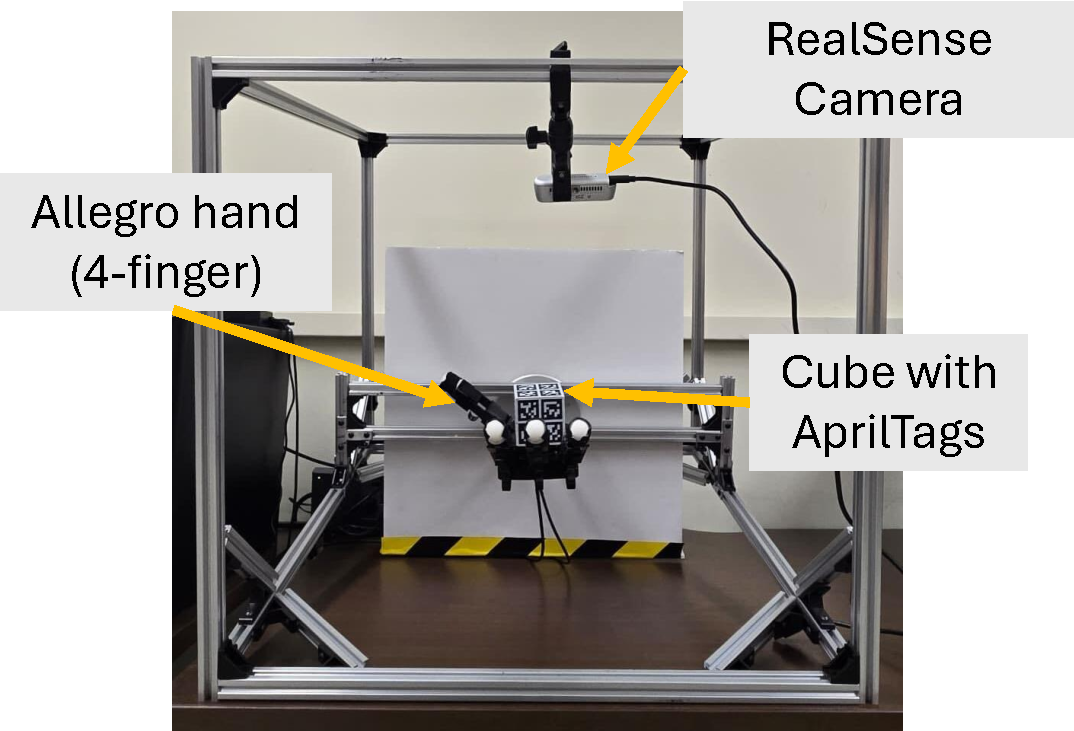
\includegraphics[width=0.5\linewidth]{figures/tasks_allegro.pdf}
\caption{Illustration of our real-world setup for the Allegro hand}
\label{fig:allegro_real_world}
\vspace{-2mm}
\end{figure}



We deploy our method on a physical Allegro Hand~\cite{allegrohand} along with a cube pose estimator based on AprilTags. The real-world setup is shown in Fig.~\ref{fig:allegro_real_world}. We evaluate in-hand cube reorientation over 10 independent trials per method. In each trial, the policy runs continuously until the cube falls off the hand. Table~\ref{tab:allegro_real_world} reports the number of consecutive successful reorientations achieved before failure across trials, along with the mean. 

\begin{table}[h]
\centering
\caption{Real-world in-hand cube reorientation on the Allegro Hand over 10 independent trials. Entries report the number of consecutive successful reorientations before failure.}
\label{tab:allegro_real_world}
\vspace{-2mm}
\scalebox{0.8}{
\begin{tabular}{lcccccccccc c}
\toprule
\textbf{Method} & \textbf{1} & \textbf{2} & \textbf{3} & \textbf{4} & \textbf{5} & \textbf{6} & \textbf{7} & \textbf{8} & \textbf{9} & \textbf{10} & \textbf{MEAN} \\
\midrule
% Baseline (Joint Control) & XX & XX & XX & XX & XX & XX & XX & XX & XX & XX & X.X \\ 
% Abhijit: Commented the baseline as I don't think we have time to finish that
UHAS (Zero-Shot)         & 0 & 1 & 1 & 1 & 0 & 1 & 0 & 0 & 2 & 2 & 0.8 \\
UHAS (Trained on Multi-Hand)         & 3 & 0 & 8 & 1 & 2 & 1 & 1 & 2 & 1 & 2 & \textbf{2.1} \\
UHAS (Trained on Allegro Hand) & 4 & 0 & 2 & 2 & 2 & 3 & 4 & 1 & 0 & 3 & \textbf{2.1} \\
\bottomrule
\end{tabular}
}
%\vspace{-2mm}
\end{table}



The Allegro-trained model achieves the highest real-world performance with a mean of 2.1 consecutive reorientations, tied with the multi-hand trained model. The zero-shot policy, however, performs substantially worse (mean 0.8), revealing a notable sim-to-real gap for cross-embodiment transfer, consistent with our LEAP Hand results. We also observe high variance across trials, with some runs reaching 8 reorientations while others fail immediately.